\cohead{\Large\textbf{Krümmung}}
\fakesubsection{Krümmung}
Wenn man sich das Schaubild als Straße aus der Vogelperspektive vorstellt, die man von links nach rechts befährt, kann man Linkskurven und Rechtskurven unterscheiden. Markiere die Links- und Rechtskurven in den folgenden Schaubildern jeweils mit verschiedenen Farben und skizziere dann die Schaubilder der Ableitungsfunktionen.\\
\begin{minipage}{\textwidth}
	\adjustbox{valign=t}{\begin{minipage}{0.24\textwidth}
			\centering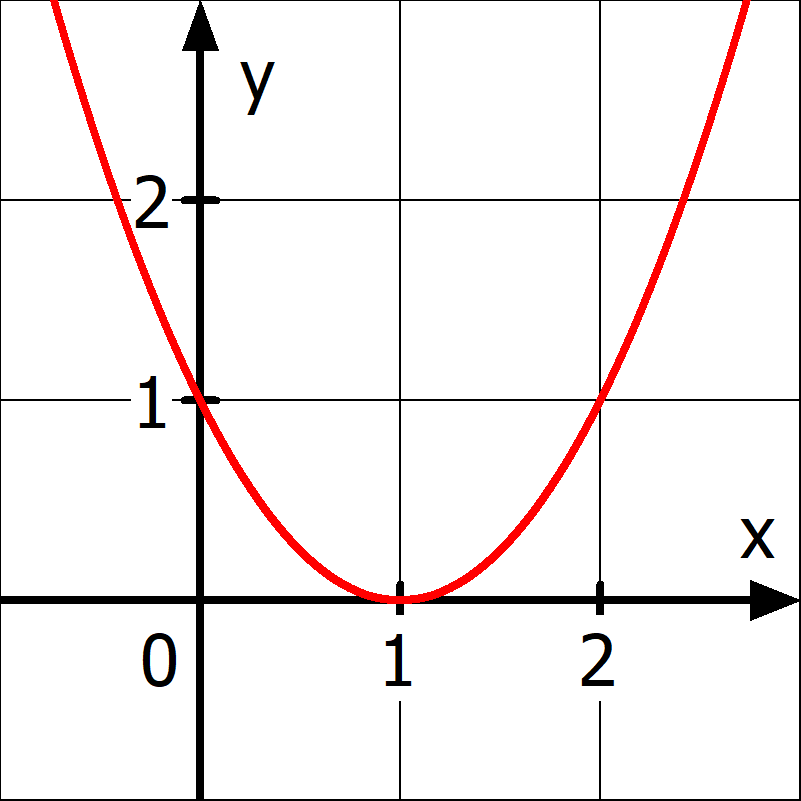
\includegraphics[width=\textwidth]{\ableitung/pics/LK1.png}
	\end{minipage}}
	\adjustbox{valign=t}{\begin{minipage}{0.24\textwidth}
			\centering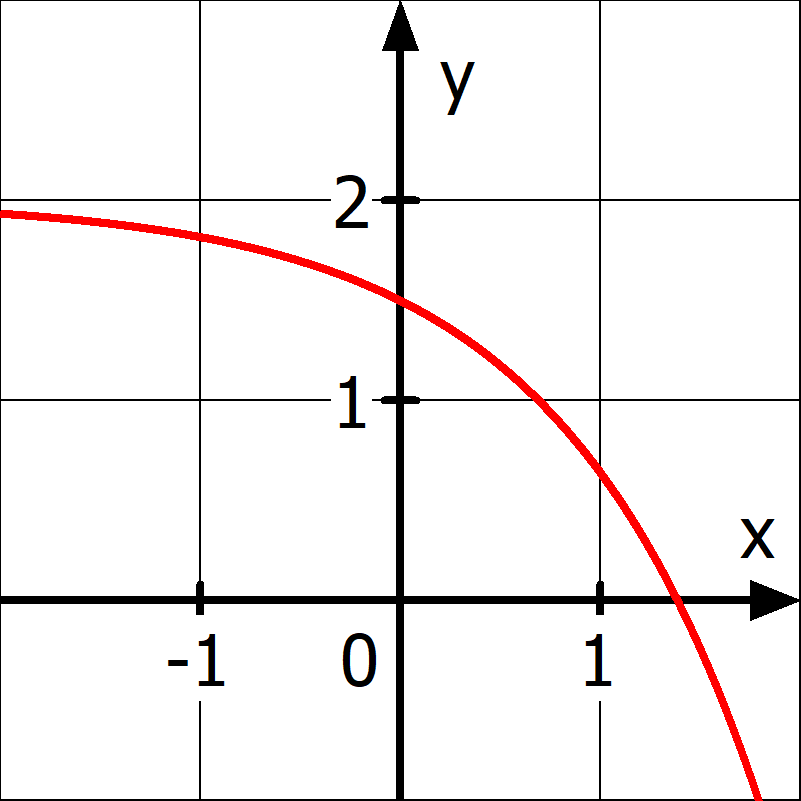
\includegraphics[width=\textwidth]{\ableitung/pics/RK1.png}
	\end{minipage}}
	\adjustbox{valign=t}{\begin{minipage}{0.24\textwidth}
			\centering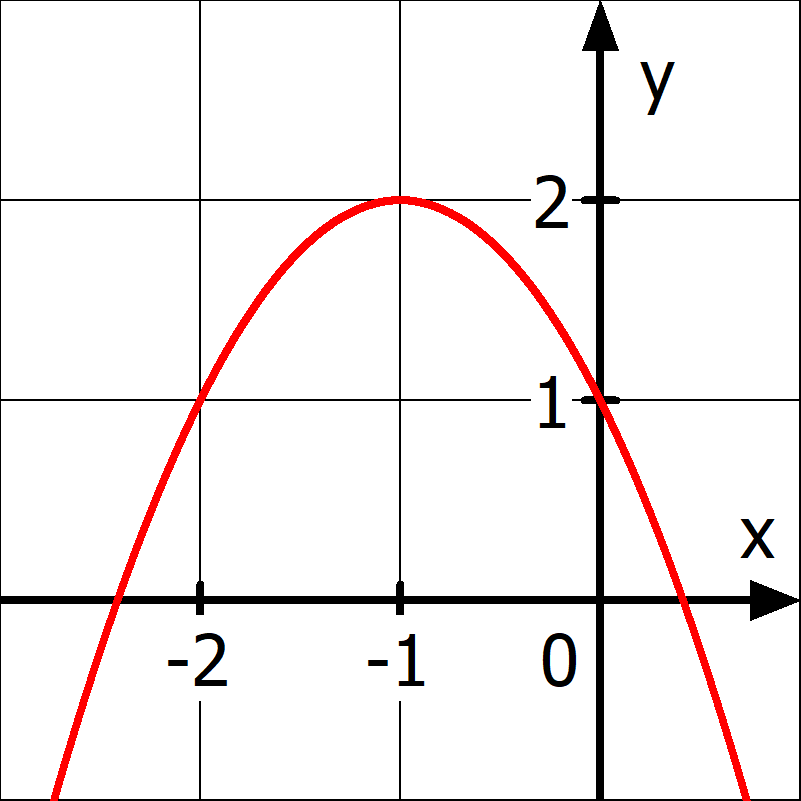
\includegraphics[width=\textwidth]{\ableitung/pics/RK2.png}
	\end{minipage}}
	\adjustbox{valign=t}{\begin{minipage}{0.24\textwidth}
			\centering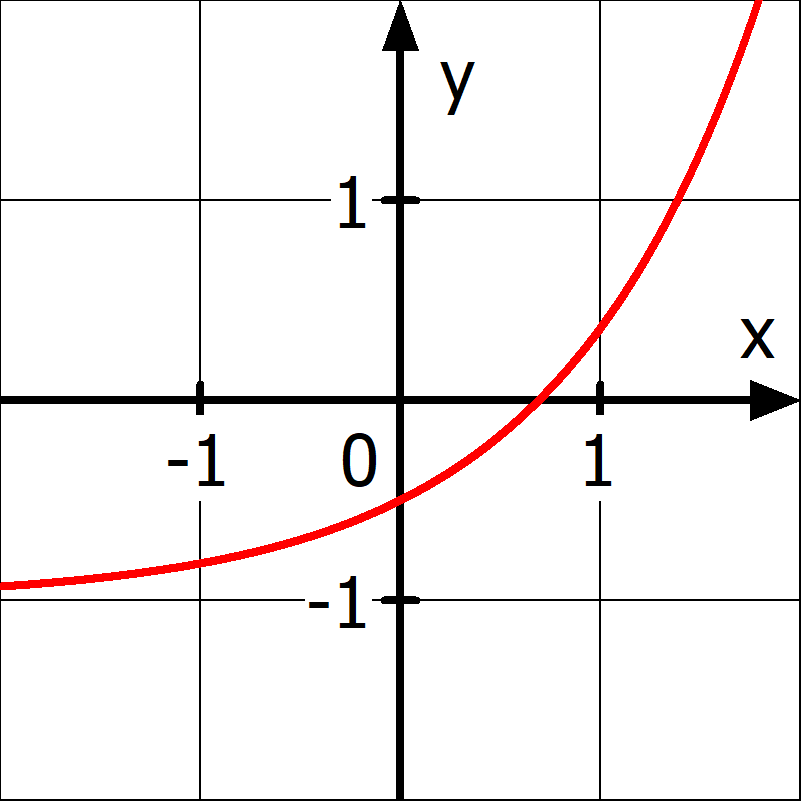
\includegraphics[width=\textwidth]{\ableitung/pics/LK2.png}
	\end{minipage}}
\end{minipage}
Schaubilder der Ableitungen:\\
\begin{minipage}{\textwidth}
	\adjustbox{valign=t}{\begin{minipage}{0.24\textwidth}
			\centering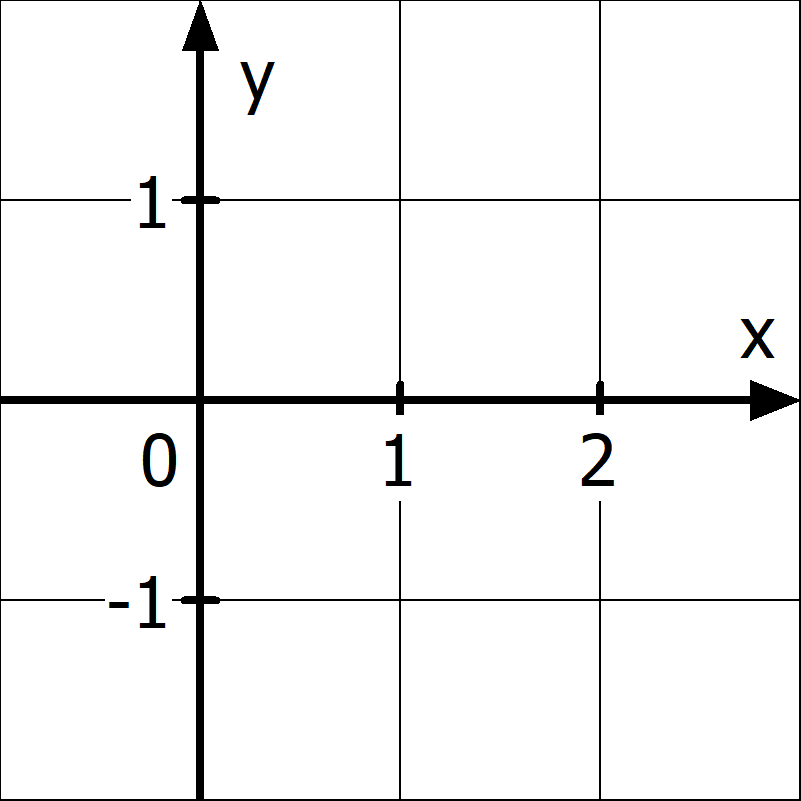
\includegraphics[width=\textwidth]{\ableitung/pics/LK1Abl.png}
	\end{minipage}}
	\adjustbox{valign=t}{\begin{minipage}{0.24\textwidth}
			\centering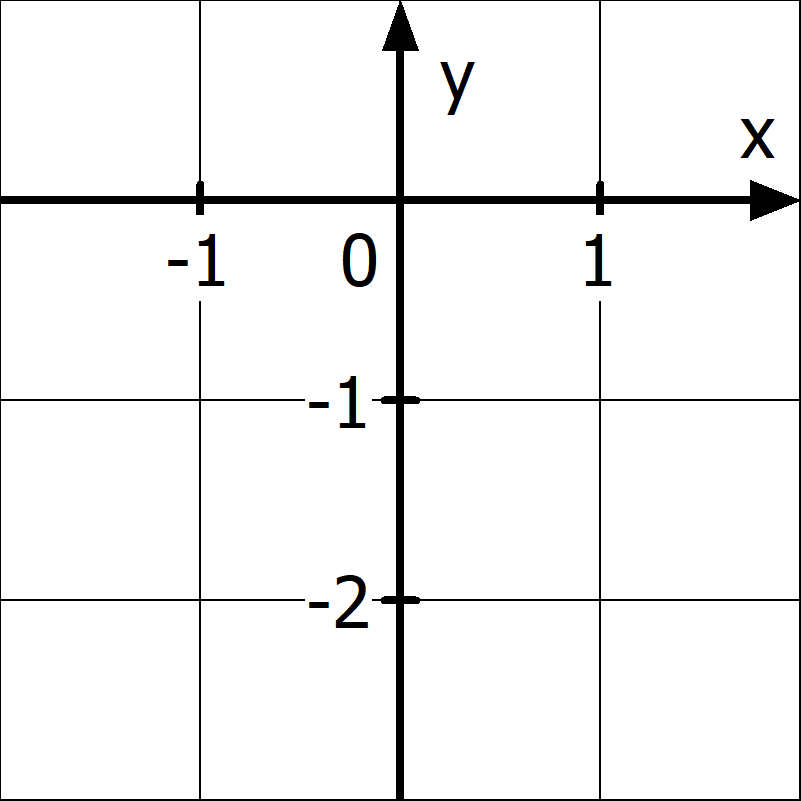
\includegraphics[width=\textwidth]{\ableitung/pics/RK1Abl.png}
	\end{minipage}}
	\adjustbox{valign=t}{\begin{minipage}{0.24\textwidth}
			\centering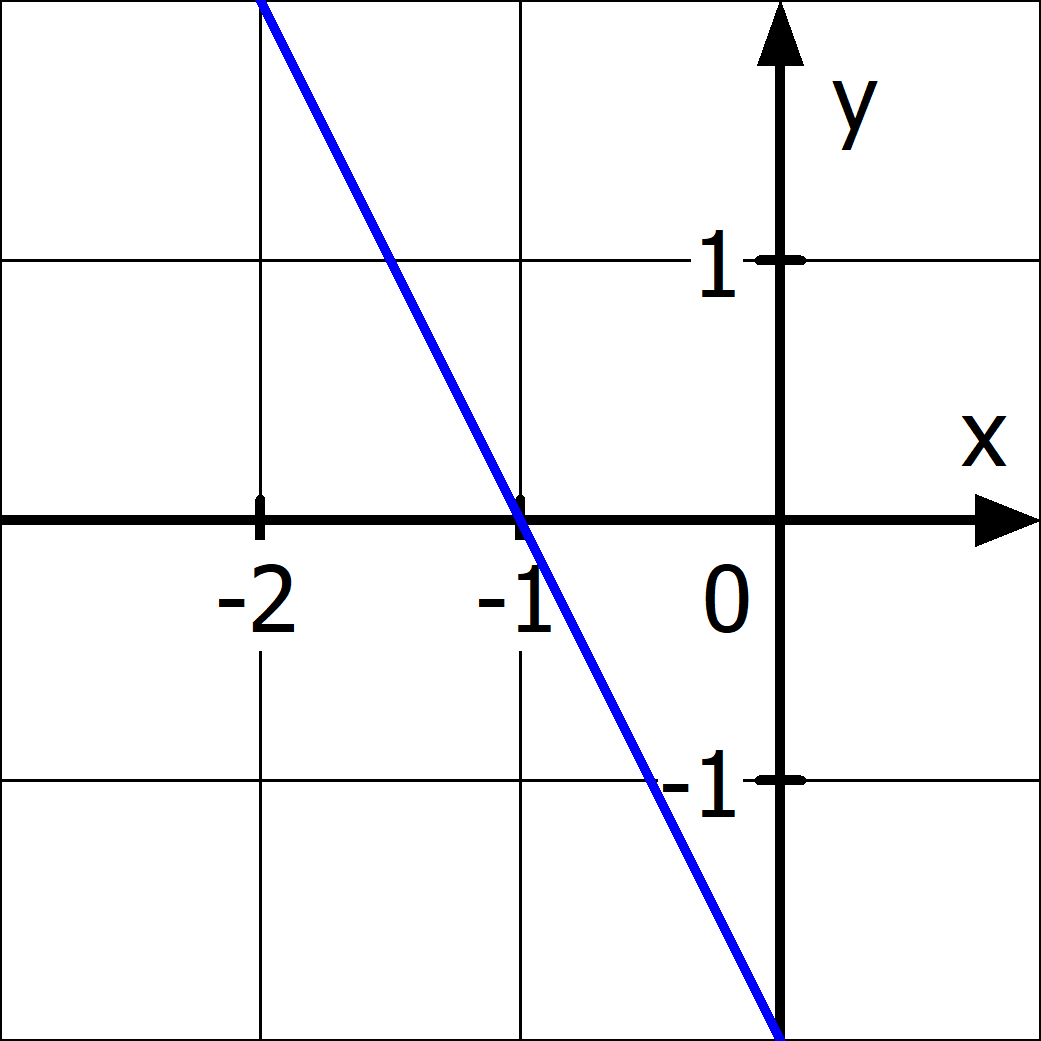
\includegraphics[width=\textwidth]{\ableitung/pics/RK2Abl.png}
	\end{minipage}}
	\adjustbox{valign=t}{\begin{minipage}{0.24\textwidth}
			\centering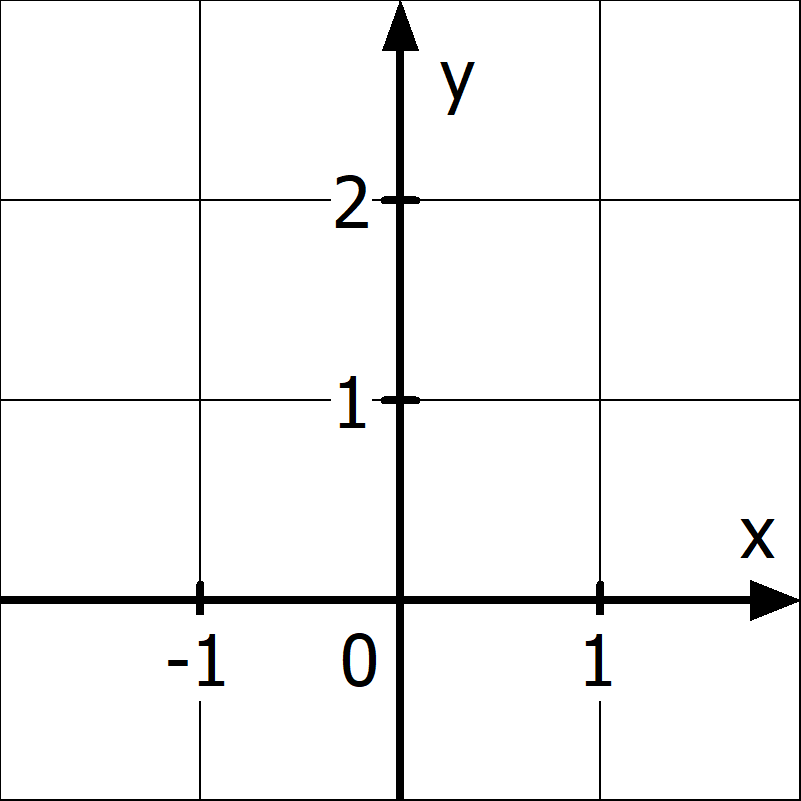
\includegraphics[width=\textwidth]{\ableitung/pics/LK2Abl.png}
	\end{minipage}}
\end{minipage}
\begin{tcolorbox}
	\textbf{Zusammenhang Krümmung und erste Ableitung:}\\
	\textcolor{loestc}{Das Schaubild von \(f(x)\) ist eine Linkskurve, genau dann wenn die Ableitung \(f'(x)\) monoton steigend ist.\\
		Das Schaubild von \(f(x)\) ist eine Rechtskurve, genau dann wenn die Ableitung \(f'(x)\) monoton fallend ist.\\}
\end{tcolorbox}
\begin{tcolorbox}
	\textbf{Zusammenhang Krümmung und zweite Ableitung:}\\
	\textcolor{loestc}{Das Schaubild von \(f(x)\) ist eine Linkskurve, genau dann wenn die zweite Ableitung \(f''(x)\) positiv ist.\\
		Das Schaubild von \(f(x)\) ist eine Rechtskurve, genau dann wenn die zweite Ableitung \(f''(x)\) negativ ist.\\}
\end{tcolorbox}
Zeige mit Hilfe der zweiten Ableitung, dass
\begin{enumerate}
	\item Das Schaubild von \(f(x)=x^2\) überall linksgekrümmt ist.
	\item Das Schaubild von \(g(x)=e^{-2x}-1\) überall rechtsgekrümmt ist.
	\item Das Schaubild von \(h(x)=x^3-3x+1\) für \(x<0\) eine Rechtskurve und für \(x>0\) eine Linkskurve vollführt.
\end{enumerate}
\newpage
%%%%%%%%%%%%%%%%%%%%%%%%%%%%%%%%%%%%%%%%%%%%%%%%%%%%%%%%%%%%%%%%%%%%%%%%%%%%%%%%%%%%%%%%%%%%%%%%%%%%%%%
\begin{Exercise}[title={\raggedright Gib mit Hilfe der zweiten Ableitung die Intervalle an, in denen das Schaubild eine Links- bzw. Rechtskurve hat.}, label=kruemmungA1]
	\begin{enumerate}[label=\alph*)]
		\item \(f_1(x)=x^3-3x^2-5x+8\)
		\item \(f_2(x)=0,5e^{-2x}+3x-4\)
		\item \(f_3(x)=-\frac{2}{3}x^3+\frac{5}{4}x^2+2x-3\)
		\item \(f_4(x)=\frac{1}{12}x^4-2x^2+5x-7\)
		\item \(f_5(x)=-3e^{2x}-3x+8\)
		\item \(f_6(x)=-x^3-9x^2-5x+6\)
		\item \(f_7(x)=-e^{-x}+x\)
		\item \(f_8(x)=0,5x^4-x^3-18x^2\)
		\item \(f_9(x)=-\frac{1}{2}x^4+7x^3-36x^2+2x-8\)
		\item \(f_{10}(x)=-\frac{1}{3}x^4-\frac{2}{3}x^3+40x^2-10x+86\)
	\end{enumerate}
\end{Exercise}
%%%%%%%%%%%%%%%%%%%%%%%%%%%%%%%%%%%%%%%%%
\begin{Answer}[ref=kruemmungA1]
	\begin{enumerate}[label=\alph*)]
		\item \(f_1(x):\) RK für \(x<1\), LK für \(x>1\)
		\item \(f_2(x):\) LK für alle \(x\in \R\)
		\item \(f_3(x):\) LK für \(x<2,5\), RK für \(x>2,5\)
		\item \(f_4(x):\) LK für \(x<-2\), RK für \(-2<x<2\), LK für \(x>2\)
		\item \(f_5(x):\) RK für alle \(x\in \R\)
		\item \(f_6(x):\) LK für \(x<-3\), RK für \(x>-3\)
		\item \(f_7(x):\) RK für alle \(x\in \R\)
		\item \(f_8(x):\) LK für \(x<-2\), RK für \(-2<x<3\), LK für \(x>3\)
		\item \(f_9(x):\) RK für \(x<3\), LK für \(3<x<4\), RK für \(x>4\)
		\item \(f_{10}(x):\) RK für \(x<-5\), LK für \(-4<x<4\), RK für \(x>4\)
	\end{enumerate}
\end{Answer}